\section{Spectrum of the BCS Hamiltonian}

\subsection{Gap Equation at Zero Temperature}

The elementary excitations over the many-body ground state \( |\psi_0\rangle \) are created by the Bogoliubov quasiparticle operators \( \gamma_{\mathbf{k},\sigma}^\dagger \). These states naturally form the eigenvectors of the diagonalized grand canonical Hamiltonian:
\[
    \hat{K}\gamma_{\mathbf{k},\sigma}^\dagger |\psi_0\rangle = (E_{\mathbf{k}} + C')\gamma_{\mathbf{k},\sigma}^\dagger |\psi_0\rangle,
\]
with the quasiparticle energy dispersion given by \( E_{\mathbf{k}} = \sqrt{\xi_k^2 + |\Delta_{\mathbf{k}}|^2} \). We are considering single quasiparticle excitations, which are the lowest-lying excited states of the system. The energy of a single quasiparticle excitation is therefore \( E_{\mathbf{k}} \) above the ground state energy \( C' \).

Consider the physical implications of this dispersion relation: whenever the momentum-dependent parameter \( \Delta_{\mathbf{k}} \neq 0 \), the excitation energy satisfies \( E_{\mathbf{k}} > 0 \) for all momenta \( \mathbf{k} \). Consequently, there exists a strictly positive energy gap between the superconducting ground state and the lowest-lying first excited state (which is determined by the global minimum of \( E_{\mathbf{k}} \)). For this fundamental reason, the function \( \Delta_{\mathbf{k}} \) is commonly referred to as the \emph{gap function}.

Recall that the gap function \( \Delta_{\mathbf{k}} \) was originally defined self-consistently through the expectation value of the pair destruction operator, \( A_{\mathbf{k}} = \langle c_{-\mathbf{k},\downarrow} c_{\mathbf{k},\uparrow} \rangle \), which looks like a self-consistency condition for the gap function: we are trying to find a solution for \( \Delta_{\mathbf{k}} \) that is consistent with the expectation value of the pair operator in the BCS ground state. The gap function is therefore determined by the microscopic details of the interaction potential \( V(\mathbf{k}, \mathbf{k}') \) and the underlying Fermi surface. Let us explicitly compute this thermodynamic average at absolute zero temperature (\( T = 0 \)), meaning we evaluate the expectation value strictly over the BCS ground state. Using the inverse Bogoliubov transformations, we express the bare particle operators in terms of the quasiparticle operators:
\[
    A_{\mathbf{k}} = \langle c_{-\mathbf{k},\downarrow} c_{\mathbf{k},\uparrow} \rangle = \left\langle \left( -v_{\mathbf{k}} \gamma_{\mathbf{k},\uparrow}^\dagger + u_{\mathbf{k}}^* \gamma_{-\mathbf{k},\downarrow} \right) \left( v_{\mathbf{k}} \gamma_{-\mathbf{k},\downarrow}^\dagger + u_{\mathbf{k}}^* \gamma_{\mathbf{k},\uparrow} \right) \right\rangle = u_{\mathbf{k}}^* v_{\mathbf{k}},
\]
where we have used the fact that \( \gamma_{\mathbf{k},\sigma} |\psi_0\rangle = 0 \). One can readily verify from the explicit definitions of the coherence factors \( u_{\mathbf{k}} \) and \( v_{\mathbf{k}} \) that their product yields:
\[
    u_{\mathbf{k}}^* v_{\mathbf{k}} = \frac{\Delta_{\mathbf{k}}}{2E_{\mathbf{k}}}.
\]
Substituting this relation back into the definition of the gap parameter, we obtain the discrete self-consistency equation:
\[
    \Delta_{\mathbf{k}} = -\frac{1}{V} \sum_{\mathbf{k}'} V(\mathbf{k}, \mathbf{k}') \frac{\Delta_{\mathbf{k}'}}{2E_{\mathbf{k}'}}.
\]
Taking the thermodynamic limit, the momentum sum transitions into an integral, yielding the celebrated BCS gap equation:
\begin{equation} \label{eq:bcs_gap_equation}
    \Delta_{\mathbf{k}} = -\int \frac{\mathrm{d}^3\mathbf{k}'}{(2\pi)^3} \frac{V(\mathbf{k}, \mathbf{k}')}{2E_{\mathbf{k}'}} \Delta_{\mathbf{k}'}.
\end{equation}
This is a non-linear integral equation for the gap function \( \Delta_{\mathbf{k}} \). Because \( E_{\mathbf{k}'} \) itself depends on \( \Delta_{\mathbf{k}'} \), it generally requires a numerical solution. However, in the physically relevant limit of weak interactions (which accurately models several conventional metallic superconductors), the gap equation can be solved analytically. This condition is realted to the many-body gap, which is essentially the \uline{energy cost to insert a single quasiparticle} into the system. We are still considering momenta in the vicinity of the Fermi surface, where the gap function is non-zero. The energy cost to insert a single quasiparticle is therefore the minimum of the dispersion \( \min_k E_{\mathbf{k}} = |\Delta_{\mathbf{k}}| \).

\subsubsection{Weak Coupling Solution for BCS Model of Interaction}

Let us first consider the effective phonon-mediated potential characteristic of a conventional superconductor. We approximate it as a separable, attractive well:
\[
    V(\mathbf{k}, \mathbf{k}') = -g w_k w_{k'},
\]
with a positive, constant coupling strength \( g = g_{e,ph}^2 > 0 \). We are implying that adding a quasiparticle to the system costs energy, and this cost is captured by this very rough mean-field approximation of the potential. The momentum dependence is captured by the step function \( w_k = \Theta(\hbar\omega_D - |\xi_k|) \), which restricts the interaction to a narrow energy shell of width \( 2\hbar\omega_D \) around the Fermi surface. Here, the kinetic energy relative to the chemical potential is \( \xi_k = \epsilon_k - \mu \). Note that the chemical potential \( \mu \) is approximately equal to the non-interacting Fermi energy \( E_F \) (the exact equality is slightly broken by the interaction, but \( \mu \simeq E_F \) holds to leading order).

To solve the integral gap equation \eqref{eq:bcs_gap_equation}, we proceed with a piecewise ansatz for the gap function that mirrors the symmetry of the potential:
\[
    \Delta_{\mathbf{k}} = \Delta_k = \Delta w_k.
\]
Substituting this ansatz and the explicit form of the interaction potential into \eqref{eq:bcs_gap_equation}, we obtain:
\[
    \Delta w_k = g \int \frac{\mathrm{d}^3\mathbf{k}'}{(2\pi)^3} \frac{w_k w_{k'} \Delta w_{k'}}{2E_{\mathbf{k}'}}.
\]
Factoring out \( \Delta w_k \) (assuming a non-trivial solution for the many body factor, \( \Delta \neq 0 \), and remembering that the dependence on \(\Delta\) is kept inside the energy denominator), the self-consistency condition simplifies to:
\[
    \frac{1}{g} = \int \frac{\mathrm{d}^3\mathbf{k}}{(2\pi)^3} \frac{\Theta(\hbar\omega_D - |\xi_k|)}{2E_k}.
\]
In the relevant region of integration specified by the Heaviside step function \( \Theta \), the quasiparticle dispersion is:
\[
    E_{\mathbf{k}} = E_k = \sqrt{\xi_k^2 + |\Delta|^2}.
\]
The minimum of this dispersion is \( \min_k E_k = |\Delta| \), which is reached exactly at the Fermi surface where \( \xi_k = 0 \) (corresponding to \( k = \sqrt{2m\mu}/\hbar \simeq k_F \)). Notice that the gap equation only dictates the modulus of the gap \( |\Delta| \), leaving the global phase undetermined. Without loss of generality, we can therefore assume \( \Delta \) to be strictly real and positive.

To evaluate the momentum integral, we transition to an energy integration for convenience by introducing the single-particle density of states \( N(\xi) \) \textit{per spin component}\footnote{We are ignoring the spin degeneracy in this discussion.} and per unit volume:
\begin{equation} \label{eq:density_of_states}
    N(\xi) = \int \frac{\mathrm{d}^3\mathbf{k}}{(2\pi)^3} \delta(\xi - \xi_k) = \frac{m^{3/2}}{\sqrt{2}\pi^2\hbar^3} \sqrt{\xi + \mu},
\end{equation}
where the last equality is obtained by explicitly evaluating the delta function integral in spherical coordinates. Physically, the density of states \( N(\xi) \) counts the number of single-particle states per unit energy interval and per unit volume. Using this definition, the gap equation transforms into:
\[
    \frac{1}{g} = \int_{-\mu}^{+\infty} d\xi \frac{N(\xi)}{2E_{\xi}} \Theta(\hbar\omega_D - |\xi|),
\]
where \( E_{\xi} = \sqrt{\xi^2 + |\Delta|^2} \), and the integral is still counting the volume of the phase space (in energy, the density of states takes the role of a weight function). Because the Debye energy is typically orders of magnitude smaller than the Fermi energy (\( \hbar\omega_D \ll E_F \approx \mu \)), the lower limit of integration \( -\mu \) can be safely replaced by the step function's cutoff \( -\hbar\omega_D \):
\[
    \frac{1}{g} = \int_{-\hbar\omega_D}^{\hbar\omega_D} d\xi \frac{N(\xi)}{2E_{\xi}}.
\]

\begin{figure}[H]
    \centering
    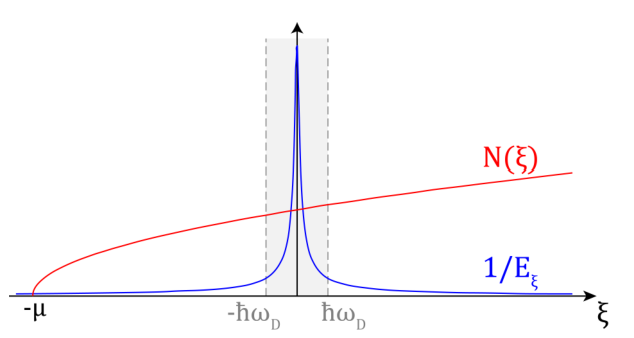
\includegraphics[width=0.8\textwidth]{img/2-bcs_density_of_states_vs_dispersion.png}
    \caption{Plot of the single-particle density of states \( N(\xi) \) and the inverse of the quasiparticle dispersion \( 1/E_\xi \), where \( E_\xi = \sqrt{\xi^2 + |\Delta|^2} \). The shaded region visually represents the narrow integration shell defined by the Debye energy cutoff \( \pm\hbar\omega_D \). Within this small window around the Fermi surface (\( \xi = 0 \)), \( 1/E_\xi \) is strongly peaked, whereas the density of states varies negligibly and can be robustly approximated by its constant value at the Fermi level, \( N_0 = N(0) \).}
    \label{fig:density_of_states_vs_dispersion}
\end{figure}

We must now carefully analyze the weak-coupling limit, where \( g \to 0 \). For the equation to hold, the right-hand side integral must correspondingly diverge towards \( +\infty \). This logarithmic divergence is only possible if the gap parameter itself vanishes, \( \Delta \to 0 \), ensuring the integrand \( 1/E_{\xi} \to \infty \) near the Fermi surface (\( \xi = 0 \)). Under these weak-coupling conditions, the function \( 1/E_{\xi} \) is extremely sharply peaked at \( \xi = 0 \) and varies rapidly over an energy scale defined by \( \Delta \) (the peak depends on the value of \( \Delta \)). Conversely, over this exact same narrow energy shell, the density of states \( N(\xi) \) is nearly constant and can be reliably approximated by its value precisely at the Fermi level, \( N_0 \equiv N(\xi=0) \). Notice that when we say \(\Delta, g \to 0\), we mean that both parameters approach zero but never actually reach it. The limit is taken in such a way that the ratio \( \Delta/g \) remains finite and well-defined.

Pulling the constant \( N_0 \) out of the integral, we evaluate the remaining expression analytically:
\[
    \frac{1}{g} = \frac{N_0}{2} \int_{-\hbar\omega_D}^{\hbar\omega_D} \frac{\mathrm{d} \xi}{\sqrt{\xi^2 + \Delta^2}} = N_0 \int_{0}^{\hbar\omega_D} \frac{1}{\Delta \sqrt{(\frac{\xi}{\Delta})^2 + 1}} \mathrm{d} \xi = N_0 \text{arcsinh}\left(\frac{\hbar\omega_D}{\Delta}\right).
\]
Inverting this relation yields:
\[
    \frac{\hbar\omega_D}{\Delta} = \sinh\left(\frac{1}{N_0 g}\right) = \frac{e^{\frac{1}{N_0 g}} - e^{-\frac{1}{N_0 g}}}{2} \sim \frac{1}{2} \exp\left(\frac{1}{N_0 g}\right),
\]
where the final asymptotic approximation relies on the behavior of \( \sinh(x) \sim e^x / 2 \) for large arguments \( x = 1/(N_0 g) \). Solving for the physical gap parameter, we obtain the seminal weak-coupling BCS result:
\begin{equation} \label{eq:bcs_gap_zero_T}
    \Delta = 2\hbar\omega_D e^{-\frac{1}{N_0 g}}.
\end{equation}

\begin{remark}
    The exponential form of \eqref{eq:bcs_gap_zero_T} carries profound physical implications. At \( T=0 \), even an infinitesimally small attractive interaction (\( g > 0 \)) is sufficient to open a finite (albeit exponentially suppressed) energy gap \( \Delta \) at the Fermi surface. Furthermore, the function \( e^{-1/(N_0 g)} \) exhibits an essential singularity at \( g=0 \). This signifies that the superconducting state cannot be reached via standard perturbative expansions starting from the non-interacting Fermi gas; the Cooper instability is a fundamentally non-perturbative phenomenon. The dimensionless parameter \( g N_0 \) acts as the effective coupling strength, which is typically quite small in conventional phonon-mediated superconductors.
\end{remark}

The fact that now we have the Debye frequency \( \omega_D \) in the prefactor of the gap equation makes this a real many-body effect. The Debye frequency is a material property that is determined by the phonon spectrum of the solid. It is not a property of the electrons themselves, but rather of the lattice vibrations, stiffness, and the speed of sound in the material (everything is then related to the mass of the ions). The fact that the gap depends on this frequency shows that the superconducting state is a collective effect that arises from the interaction between electrons and the lattice vibrations.

\subsubsection{Weak Coupling Solution for Ultracold Fermi Gases}

We now shift our focus to ultracold Fermi gases, where the effective interaction is characterized by a short-range contact potential. In momentum space, this is modeled as \( V(\mathbf{k}, \mathbf{k}') = v_0 w_k w_{k'} \), with the cutoff function \( w_k = \Theta(k_0 - k) \).\TODO{add image of omega as cutoff function} We are physically interested in the limit where the ultraviolet cutoff momentum is taken to infinity, \( k_0 \to \infty \). To ensure physical observables remain well-defined, the bare coupling strength \( v_0 \) must be simultaneously rescaled (renormalized) in order to hold the low-energy \( s \)-wave scattering length \( a \) constant.

Applying the same piecewise ansatz for the gap function, \( \Delta_{\mathbf{k}} = \Delta_k = \Delta w_k \), the generalized gap equation \eqref{eq:bcs_gap_equation} becomes:
\[
    \Delta w_k = -v_0 \int \frac{\mathrm{d}^3\mathbf{k}'}{(2\pi)^3} \frac{w_k w_{k'} \Delta w_{k'}}{2E_{k'}}.
\]
From now on we repeat the same computation done for the superconducing case. Dividing by \( \Delta w_k \) yields the bare relation:
\[
    -\frac{1}{v_0} = \int \frac{\mathrm{d}^3\mathbf{k}}{(2\pi)^3} \frac{w_k^2}{2E_k}.
\]
To eliminate the divergent bare coupling \( v_0 \) in favor of the physical scattering length \( a \), we formally add and subtract an identical free-particle integral containing the bare kinetic energy \( \epsilon_k = \hbar^2 k^2 / (2m) \):
\[
    -\frac{1}{v_0} = \int \frac{\mathrm{d}^3\mathbf{k}}{(2\pi)^3} \left( \frac{1}{2E_k} - \frac{1}{2\epsilon_k} \right) w_k^2 + \int \frac{\mathrm{d}^3\mathbf{k}}{(2\pi)^3} \frac{w_k^2}{2\epsilon_k}.
\]
We recognize that the bare coupling and the last integral term are exactly related by the Lippmann-Schwinger equation for the \( T \)-matrix at zero energy, which defines the running of \( v_0 \) with the scattering length \( a \):
\[
    -\frac{m}{4\pi\hbar^2 a} = \int \frac{\mathrm{d}^3\mathbf{k}}{(2\pi)^3} \left( \frac{1}{2E_k} - \frac{1}{2\epsilon_k} \right) w_k^2.
\]
Because the integrand in the parenthesis now scales as \( k^{-4} \) for large momenta, the integral is explicitly ultraviolet convergent. We can therefore safely remove the artificial regularization by taking the limit \( k_0 \to \infty \), yielding the fully regularized gap equation:
\begin{equation} \label{eq:ultracold_gap_regularized}
    -\frac{m}{4\pi\hbar^2 a} = \int \frac{\mathrm{d}^3\mathbf{k}}{(2\pi)^3} \left( \frac{1}{2E_k} - \frac{1}{2\epsilon_k} \right).
\end{equation}

This convergent integral can be evaluated analytically in terms of complete elliptic integrals. Let us consider the specific regime of a weak attractive interaction, characterized by a small and negative scattering length \( a \to 0^- \). In this BCS-like limit, the chemical potential approaches the non-interacting Fermi energy (\( \mu \simeq E_F \)) and the gap is small (\( \Delta \ll \mu \)). The regularized integration yields the explicit asymptotic solution:
\begin{equation} \label{eq:ultracold_gap_result}
    \Delta = \frac{8E_F}{e^2} e^{\frac{\pi}{2 k_F a}}.
\end{equation}
This profound result explicitly dictates how the pairing gap becomes exponentially suppressed in the limit \( k_F a \to 0^- \). Physically, adding particles to the system costs energy, and this cost is captured by this very rough mean-field approximation of the potential. The gap is exponentially small in the weak-coupling limit, but it is non-zero for any finite attractive interaction, indicating that the system is unstable.

It is structurally insightful to compare this ultracold gas result with the solid-state BCS expression \eqref{eq:bcs_gap_zero_T}. Recall that the 3D density of states at the Fermi surface is \( N_0 = (m k_F)/(2\pi^2\hbar^2) \). If we identify the effective BCS coupling parameter with the first-order Born approximation of the scattering amplitude, \( g = -4\pi\hbar^2 a / m \), the exponential dependence \( e^{\pi/(2 k_F a)} \) strictly coincides with the BCS term \( e^{-1/(N_0 g)} \). This mapping perfectly reproduces the exponent; however, retaining the full \( 1/(2\epsilon_k) \) counter-term in the integral regularization—rather than relying strictly on the lowest-order Born approximation—is mathematically critical for capturing the exact \( 8/e^2 \) numerical prefactor governing the overall energy scale of the pairing gap.

\subsubsection{Comparison with Spectrum of the Weak Interacting Bose Gas}

In the case of a weakly interacting Bose gas, the spectrum of elementary excitations is determined by the Bogoliubov dispersion relation:...\TODO{complete, graph and compare}

[drawing of ``BCS wavefunction'' as a product of pairs of fermions in momentum space, with arrows indicating the pairing of opposite momenta and spins]

In order to create an excitation, we have to add momenta to an electron inside a cooper pair, but this cannot be done continuously because the two electrons are bound together. The energy cost to break a pair is the gap \( \Delta \). In contrast, in a weakly interacting Bose gas, the Bogoliubov spectrum is gapless, and excitations can be created with arbitrarily small energy by adding small momenta to the condensate. This fundamental difference in the excitation spectrum leads to distinct physical properties between fermionic superfluids and bosonic condensates.

the cooper pairs can be broke releasing energy or absorbing energy interacting with the phonons (we have ignored them for a while but they are still in the description).

transition to the landau criterion...

\subsection{Elementary Excitations and Landau Criterion}

All the excited states of the grand-canonical Hamiltonian \( \hat{K} \) are systematically obtained by acting with the quasiparticle creation operator \( \gamma_{\mathbf{k},\sigma}^\dagger \) on the many-body ground state \( |\psi_0(\mu)\rangle \). The energy dispersion of these elementary excitations in a BCS superconductor or superfluid is thus given by \( E_k = \sqrt{\xi_k^2 + |\Delta|^2} \).

resistivity in superconductors (zero and then \(T^3\), \(\rho\) vs \(T\) graph), graph and analogy with superfluid \TODO{complete paragraph}

\TODO{add image of a dispersion curve showing excitation energy versus momentum, with a minimum gap at the Fermi momentum, illustrating the Landau criterion geometry}

Applying the Landau criterion for superfluidity to this specific dispersion relation \( E_k \), we look for the minimum of \( E_k/k \). One finds a strictly positive critical velocity \( v_c > 0 \) (where \( v_c \simeq \Delta/(\hbar k_F) \) in the physically relevant regime where \( \Delta \ll E_F \)). We thus conclude that the combination of BCS theory and the Landau kinematic criterion rigorously predicts that a Fermi gas with an attractive interaction fundamentally behaves as a superfluid (if the particles are neutral) or a superconductor (if the particles are charged) at absolute zero temperature \( T = 0 \).

\subsubsection{Momentum Distribution Function}

The average number of fermions with momentum \( \mathbf{k} \) and spin \( \sigma \) in the ground state \( |\psi_0\rangle \) (at \( T = 0 \)) is defined by the expectation value of the bare number operator:
\[
    n_{\mathbf{k},\sigma} = \langle c_{\mathbf{k},\sigma}^\dagger c_{\mathbf{k},\sigma} \rangle.
\]
Cite time of flight experiments: release an ultracold Fermi gas from the trap and let it expand freely, if particles are independent their final position is proportional to their initial momentum, and the density of particles in the final position is proportional to the momentum distribution function. This is a direct measurement of the momentum distribution function...

show now graph of the momentum distribution function, as a theta function for a non-interacting Fermi gas, and say tht we should obtain the same result out of the small window around the Fermi surface, where we will see the true effect of the emergent many-body physics of the BCS state. \TODO{add graph and explain}

To evaluate this, we utilize the inverse Bogoliubov transformations, which explicitly dictate the relations between the bare particle operators \( c_{\mathbf{k},\sigma}, c_{\mathbf{k},\sigma}^\dagger \) and the Bogoliubov quasiparticle operators \( \gamma_{\mathbf{k},\sigma}, \gamma_{\mathbf{k},\sigma}^\dagger \):
\[
    c_{\mathbf{k},\uparrow} = u_{\mathbf{k}}^* \gamma_{\mathbf{k},\uparrow} + v_{\mathbf{k}} \gamma_{-\mathbf{k},\downarrow}^\dagger,
\]
\[
    c_{\mathbf{k},\downarrow} = u_{\mathbf{k}}^* \gamma_{\mathbf{k},\downarrow} - v_{\mathbf{k}} \gamma_{-\mathbf{k},\uparrow}^\dagger.
\]
Taking the Hermitian conjugate yields the corresponding creation operators:
\[
    c_{\mathbf{k},\uparrow}^\dagger = u_{\mathbf{k}} \gamma_{\mathbf{k},\uparrow}^\dagger + v_{\mathbf{k}}^* \gamma_{-\mathbf{k},\downarrow},
\]
\[
    c_{\mathbf{k},\downarrow}^\dagger = u_{\mathbf{k}} \gamma_{\mathbf{k},\downarrow}^\dagger - v_{\mathbf{k}}^* \gamma_{-\mathbf{k},\uparrow}.
\]
Because the BCS ground state is defined as the quasiparticle vacuum (\( \gamma_{\mathbf{k},\sigma} |\psi_0\rangle = 0 \)), only the terms involving normal-ordered quasiparticle operators contribute to the expectation value. We thus have:
\[
    \langle c_{\mathbf{k},\uparrow}^\dagger c_{\mathbf{k},\uparrow} \rangle = \langle (v_{\mathbf{k}}^* v_{\mathbf{k}} \gamma_{-\mathbf{k},\downarrow} \gamma_{-\mathbf{k},\downarrow}^\dagger) \rangle = |v_{\mathbf{k}}|^2,
\]
\[
    \langle c_{\mathbf{k},\downarrow}^\dagger c_{\mathbf{k},\downarrow} \rangle = \langle (-v_{\mathbf{k}}^*)(-v_{\mathbf{k}}) \gamma_{-\mathbf{k},\uparrow} \gamma_{-\mathbf{k},\uparrow}^\dagger \rangle = |v_{\mathbf{k}}|^2.
\]
Recalling the explicit analytical expression for the coherence factor \( v_{\mathbf{k}} \), one obtains the momentum distribution:
\begin{equation} \label{eq:momentum_distribution}
    n_{\mathbf{k},\sigma} = |v_{\mathbf{k}}|^2 = \frac{1}{2} \left( 1 - \frac{\xi_k}{E_k} \right).
\end{equation}

\TODO{add image of a plot showing the momentum distribution function as a function of momentum, displaying a smeared Fermi step near the Fermi momentum}

We now note that in the weak-coupling regime where \( \Delta \ll E_F \), the pairing gap is much smaller than the relative kinetic energy \( |\xi_k| \), except within a very narrow momentum window (of order of a few \( (m\Delta)/(\hbar^2 k_F) \)) centered directly around the Fermi momentum \( k_F \). Outside this specific window, the dispersion smoothly approximates the absolute value of the kinetic energy, \( E_k \approx |\xi_k| \). Consequently, the distribution sharply approaches \( n_{\mathbf{k},\sigma} \simeq 1 \) for states deep inside the Fermi sea, or \( n_{\mathbf{k},\sigma} \simeq 0 \) for states far above it, depending entirely on the sign of \( \xi_k \). One thus naturally recovers a momentum distribution which essentially coincides with the standard Heaviside step distribution of an ideal non-interacting Fermi gas at \( T = 0 \), with the crucial modification of a continuous smearing confined to a small momentum window around \( k_F \).

We did not show why this expression results in a smearing around the small energy window around \(k_F\), but this can be seen by explicitly giving a functional form to \(\Delta\), since it is the crucial parameter that determines the width of the smearing.

\subsection{Gap Equation at Finite Temperature}

When calculating the pairing amplitude \( \langle c_{-\mathbf{k},\downarrow} c_{\mathbf{k},\uparrow} \rangle \) (or similar expectation values for the momentum distribution) at absolute zero temperature \( T = 0 \) in the previous section, we heavily utilized the property that the ground state is perfectly annihilated by the quasiparticle destruction operator \( \gamma_{\mathbf{k},\sigma} \), leading to \( \langle \gamma_{\mathbf{k},\sigma}^\dagger \gamma_{\mathbf{k},\sigma} \rangle = 0 \).

At any finite temperature \( T > 0 \), the pure ground state expectation average must be rigorously replaced by the statistical thermal average in the grand-canonical ensemble. In this thermodynamic trace, we can safely drop the constant energy offset term \( C' \) since it identically cancels between the numerator and denominator of the thermal average formula. We are thus left evaluating thermodynamics with the diagonalized grand-canonical Hamiltonian \( \hat{K}' = \sum_{\mathbf{k},\sigma} E_{\mathbf{k}} \gamma_{\mathbf{k},\sigma}^\dagger \gamma_{\mathbf{k},\sigma} \).

\begin{remark}
    Notice that \( \hat{K}' \) formally coincides with the Hamiltonian of an ideal, non-interacting Fermi gas, with the critical distinction that the non-interacting kinetic energy \( \xi_k = \epsilon_k - \mu \) is replaced by the superconducting quasiparticle dispersion \( E_{\mathbf{k}} \).
\end{remark}

With this direct structural identification, we conclude immediately that at finite temperature, the average number of thermally excited elementary excitations is governed by the standard Fermi-Dirac distribution:
\[
    \langle \gamma_{\mathbf{k},\sigma}^\dagger \gamma_{\mathbf{k},\sigma} \rangle = f(E_{\mathbf{k}}) = \frac{1}{e^{\beta E_{\mathbf{k}}} + 1},
\]
where \( \beta = 1/(k_B T) \).

\TODO{add image of a schematic plot showing the typical behavior of the superconducting gap order parameter as a function of temperature, continuously decreasing to zero at the critical temperature}

We thus re-evaluate the anomalous pair expectation value at finite temperature using the Bogoliubov transformations and the Fermi-Dirac statistics:
\[
    \langle c_{-\mathbf{k},\downarrow} c_{\mathbf{k},\uparrow} \rangle = \left\langle \left( -v_{\mathbf{k}} \gamma_{\mathbf{k},\uparrow}^\dagger + u_{\mathbf{k}}^* \gamma_{-\mathbf{k},\downarrow} \right) \left( u_{\mathbf{k}}^* \gamma_{\mathbf{k},\uparrow} + v_{\mathbf{k}} \gamma_{-\mathbf{k},\downarrow}^\dagger \right) \right\rangle
\]
\[
    = -v_{\mathbf{k}} u_{\mathbf{k}}^* \langle \gamma_{\mathbf{k},\uparrow}^\dagger \gamma_{\mathbf{k},\uparrow} \rangle + u_{\mathbf{k}}^* v_{\mathbf{k}} \langle \gamma_{-\mathbf{k},\downarrow} \gamma_{-\mathbf{k},\downarrow}^\dagger \rangle
\]
\[
    = -v_{\mathbf{k}} u_{\mathbf{k}}^* f(E_{\mathbf{k}}) + u_{\mathbf{k}}^* v_{\mathbf{k}} [1 - f(E_{\mathbf{k}})]
\]
\[
    = u_{\mathbf{k}}^* v_{\mathbf{k}} [1 - 2f(E_{\mathbf{k}})].
\]
Using the algebraic identity \( 1 - 2f(x) = \tanh(x/2) \) for the Fermi-Dirac function, this simplifies elegantly to:
\[
    \langle c_{-\mathbf{k},\downarrow} c_{\mathbf{k},\uparrow} \rangle = u_{\mathbf{k}}^* v_{\mathbf{k}} \tanh\left(\frac{\beta E_{\mathbf{k}}}{2}\right).
\]

By inserting this temperature-dependent expectation value back into the fundamental definition of the gap function and taking the standard thermodynamic limit, we obtain the generalized gap equation at finite temperature:
\begin{equation} \label{eq:finite_t_gap_equation}
    \Delta_{\mathbf{k}} = -\int \frac{\mathrm{d}^3\mathbf{k}'}{(2\pi)^3} \frac{V(\mathbf{k}, \mathbf{k}')}{2E_{\mathbf{k}'}} \tanh\left(\frac{\beta E_{\mathbf{k}'}}{2}\right) \Delta_{\mathbf{k}'}.
\end{equation}

Specifying this to the case of a conventional superconductor utilizing the separable BCS model interaction, and introducing again the density of states \( N(\xi) \), one integrates out the angular dependence to find:
\[
    \frac{1}{g} = \int_{-\hbar\omega_D}^{\hbar\omega_D} d\xi \frac{N(\xi)}{2E_{\xi}} \tanh\left(\frac{\beta E_{\xi}}{2}\right).
\]
Just as in the zero-temperature derivation, for a weak-coupling superconductor where \( \Delta \ll E_F \), the density of states \( N(\xi) \) can be accurately approximated as a constant equal to its value exactly at the Fermi level, \( N(\xi) \approx N_0 \). In this way, the integral equation further reduces to:
\[
    \frac{1}{g} = N_0 \int_{0}^{\hbar\omega_D} d\xi \frac{1}{E_{\xi}} \tanh\left(\frac{\beta E_{\xi}}{2}\right).
\]

In general, there exists no closed-form analytic solution for this non-linear integral equation (even in the strict limit where \( g \to 0 \)), meaning the full temperature dependence \( \Delta(T) \) must typically be solved numerically. The typical numerical solution exhibits the standard behavior of an order parameter in a second-order phase transition: it monotonically decreases from its zero-temperature value and vanishes continuously at a specific critical temperature \( T_c \).

However, in the weak-coupling limit, powerful analytic asymptotic expressions can be derived for specific temperature regimes. At very low temperatures, \( T \ll T_c \ll T_F \), the gap exponentially approaches its zero-temperature value \( \Delta_0 \equiv \Delta(T=0) \) according to:
\[
    \Delta(T) = \Delta_0 \left[ 1 - \left(\frac{2\pi k_B T}{\Delta_0}\right)^{\frac{1}{2}} e^{-\frac{\Delta_0}{k_B T}} \right].
\]
Conversely, very close to the critical phase transition, in the Ginzburg-Landau regime where \( (T_c - T)/T_c \ll 1 \), the gap closes with a characteristic square-root scaling:
\[
    \Delta(T) = 3.06 k_B T_c \left(1 - \frac{T}{T_c}\right)^{\frac{1}{2}},
\]
where the specific universal numerical prefactor is derived from the Riemann zeta function, i.e.
\[
    \pi \left( \frac{8}{7\zeta(3)} \right)^{1/2} \simeq 3.06.
\]

In a completely analogous manner, utilizing the contact interaction regularized by the scattering length \( a \), the finite-temperature gap equation for an ultracold attractive Fermi gas reads:
\begin{equation} \label{eq:ultracold_finite_t_gap}
    -\frac{m}{4\pi a} = \int \frac{\mathrm{d}^3\mathbf{k}}{(2\pi)^3} \left[ \frac{\tanh(\beta E_k / 2)}{2E_k} - \frac{1}{2\epsilon_k} \right].
\end{equation}
Through rigorous analysis, it can be mathematically shown that the exact same asymptotic expansions—both the exponential correction at low \( T \) and the square-root scaling close to \( T_c \)—are valid for the ultracold gas as well, provided that the appropriate zero-temperature gap value \( \Delta_0 \) characteristic of the contact potential is consistently used.

\subsection{Critical Temperature}

As the temperature approaches the critical temperature from below (\( T \to T_c^- \)), the superconducting order parameter vanishes, \( \Delta(T) \to 0 \), and the quasiparticle dispersion seamlessly reduces to the absolute value of the normal state kinetic energy, \( E_\xi \to |\xi| \). Consequently, the finite-temperature gap equation simplifies considerably:
\[
    \frac{1}{N_0 g} = \int_0^{\hbar\omega_D} d\xi \frac{1}{\xi} \tanh\left(\frac{\beta_c \xi}{2}\right),
\]
where \( \beta_c = (k_B T_c)^{-1} \). By introducing the dimensionless integration variable \( x = \beta_c \xi / 2 \), the equation can be systematically evaluated using integration by parts:
\[
    \begin{aligned}
        \frac{1}{N_0 g} & = \int_0^{\frac{\hbar\omega_D}{2k_B T_c}} dx \frac{\tanh(x)}{x}                                                                              \\
                        & = \left[ \ln(x) \tanh(x) \right]_0^{\frac{\hbar\omega_D}{2k_B T_c}} - \int_0^{\frac{\hbar\omega_D}{2k_B T_c}} dx \frac{\ln(x)}{(\cosh(x))^2} \\
                        & \simeq \ln\left( \frac{\hbar\omega_D}{2k_B T_c} \right) - \int_0^\infty dx \frac{\ln(x)}{(\cosh(x))^2}                                       \\
                        & = \ln\left( \frac{\hbar\omega_D}{2k_B T_c} \right) + \ln\left( \frac{4e^\gamma}{\pi} \right)                                                 \\
                        & = \ln\left( \frac{2\hbar\omega_D e^\gamma}{\pi k_B T_c} \right).
    \end{aligned}
\]
In moving from the exact integration by parts to the asymptotic approximation, we have safely extended the upper limit of the second integral to infinity. This is physically justified because \( k_B T_c \) is expected to be on the same order of magnitude as the zero-temperature gap \( \Delta_0 \), which is strictly much smaller than the Debye energy cutoff \( \hbar\omega_D \) in the weak-coupling limit (\( k_B T_c \ll \hbar\omega_D \)). The numerical constant \( \gamma \approx 0.577216 \) is the Euler-Mascheroni constant.

Inverting this logarithmic relation yields an explicit expression for the critical temperature:
\[
    k_B T_c = \frac{2\hbar\omega_D e^\gamma}{\pi} e^{-\frac{1}{g N_0}} = \frac{e^\gamma}{\pi} \Delta_0.
\]
We have thus analytically obtained a fundamental universal ratio connecting the zero-temperature pairing gap to the critical temperature:
\begin{equation} \label{eq:bcs_universal_ratio}
    \frac{2\Delta_0}{k_B T_c} = \frac{2\pi}{e^\gamma} \approx 3.53.
\end{equation}

This ratio is considered universal because it does not depend on the specific microscopic details of the attractive interaction, provided the system remains strictly in the weak-coupling regime. Experimental measurements of this ratio across numerous conventional "weak-coupling" superconductors have spectacularly confirmed this precise theoretical prediction of BCS theory.

We also observe that the critical temperature \( T_c \) (identically to the zero-temperature gap \( \Delta_0 \)) is directly proportional to the Debye frequency \( \omega_D \). Because the lattice vibration frequencies scale inversely with the square root of the ionic mass, \( \omega_D \propto 1/\sqrt{M} \), this proportionality perfectly explains the experimentally observed isotope effect. The critical temperature predictably shifts when the constituent lattice ions are replaced by heavier or lighter equivalent isotopes. This historically crucial experimental finding was one of the earliest direct indications that phonons must play the central role in mediating superconductivity, as equivalent isotopes form identical electronic band structures but critically modify the background phonon frequencies. The exact prediction \( T_c \propto 1/\sqrt{M} \) has been robustly verified in several conventional superconductors.

Furthermore, for ultracold Fermi gases governed by a zero-range contact potential, the finite-temperature gap equation identically reduces at \( T_c \) to:
\[
    -\frac{m}{4\pi a} = \int \frac{d^3k}{(2\pi)^3} \left[ \frac{\tanh(\beta_c \xi_k / 2)}{2\xi_k} - \frac{1}{2\epsilon_k} \right].
\]
By evaluating this integral in the weak-coupling BCS limit where \( k_F a \to 0^- \), one obtains an analytic expression for \( T_c \), proving that the universal ratio \( 2\Delta_0 / (k_B T_c) \approx 3.53 \) remains perfectly valid in this entirely different physical system, utilizing the appropriate contact potential zero-temperature gap \( \Delta_0 \).

\subsection{Low Temperature Expansion for the Specific Heat}

Let us investigate the thermodynamic energy difference \( \delta E(T) = E(T) - E(0) \) between the total energy of the superconducting system at a finite temperature \( T \) and its absolute zero ground state. We can calculate \( \delta E(T) \) directly by recalling that \( E_k \) describes the energy dispersion of the independent elementary excitations (Bogoliubov quasiparticles). Because these quasiparticles are fermions, their thermal occupation is strictly governed by the Fermi-Dirac distribution function \( f(E_k) \). The chemical potential for these elementary excitations is set to zero, since their average number is not an independently conserved thermodynamic variable, but rather fluctuates dynamically as a function of temperature. One thus has:
\[
    \delta E(T) = 2V \int \frac{d^3k}{(2\pi)^3} E_k f(E_k) = 2V \int_{-\mu}^{+\infty} N(\xi) E_\xi f(E_\xi) d\xi.
\]

We now focus specifically on the extreme low-temperature limit, where the thermal energy is drastically smaller than the pairing gap, \( k_B T \ll \Delta(T) \simeq \Delta_0 \). In this strongly suppressed regime, the Fermi-Dirac distribution effectively reduces to the classical Maxwell-Boltzmann exponential tail:
\[
    f(E_\xi) = \frac{1}{e^{\beta E_\xi} + 1} \simeq e^{-\beta E_\xi}.
\]
This exponential decay in the integrand severely restricts the relevant region of integration to a very narrow band where the kinetic energy \( |\xi| \) is less than a few \( k_B T \), which itself is much smaller than the Fermi energy \( E_F \). Within this highly restricted region, we can confidently approximate the density of states as a constant evaluated at the Fermi level, \( N(\xi) \simeq N_0 \). Furthermore, for energies outside the exponential function, we approximate \( E_\xi \simeq \Delta \), while within the exponential we retain the quadratic expansion of the quasiparticle dispersion \( E_\xi \simeq \Delta(1 + \xi^2/(2\Delta^2)) \). This yields:
\[
    \frac{\delta E(T)}{V} = 2N_0 \Delta e^{-\beta\Delta} \int_{-\infty}^{+\infty} e^{-\beta\xi^2/(2\Delta)} d\xi = 2N_0 \Delta^2 e^{-\beta\Delta} \sqrt{\frac{2\pi}{\beta\Delta}}.
\]

The specific heat capacity at constant volume, \( C_V \), is then obtained by differentiating this internal energy with respect to temperature:
\[
    \begin{aligned}
        \frac{C_V}{V} & = \frac{\partial E(T)}{\partial T} = \frac{\partial \delta E(T)}{\partial T} = -k_B \beta^2 \frac{\partial E(\beta)}{\partial \beta} \\
                      & = 2k_B N_0 (\beta\Delta)^2 \Delta \sqrt{\frac{2\pi}{\beta\Delta}} e^{-\beta\Delta} + \text{sub-leading terms}.
    \end{aligned}
\]

\TODO{add image of a plot comparing the specific heat versus temperature for a superconductor exhibiting exponential behavior and a normal Fermi liquid exhibiting linear behavior}

The sub-leading terms can be safely disregarded in the strict limit \( k_B T \ll \Delta \). These neglected terms include contributions containing the temperature derivative of the gap itself, \( \partial\Delta(T)/\partial T \). Because the low-temperature expansion of the gap parameter \( \Delta(T) \) exhibits an exponentially suppressed deviation from \( \Delta_0 \), its derivative is identically exponentially suppressed and non-dominant. We can thus consistently set \( \Delta = \Delta_0 \) in the prefactors to obtain the final leading-order expression for the low-temperature specific heat:
\begin{equation} \label{eq:bcs_specific_heat}
    \frac{C_V}{V} = 2k_B N_0 \sqrt{2\pi} \Delta_0 \left( \frac{\Delta_0}{k_B T} \right)^{\frac{3}{2}} e^{-\frac{\Delta_0}{k_B T}}.
\end{equation}

We clearly observe that the specific heat vanishes exponentially as \( T \to 0 \). This dramatic exponential suppression is a direct macroscopic consequence of the finite energy gap in the quasiparticle dispersion spectrum, effectively freezing out thermal excitations at low temperatures. This stands in sharp contrast to the characteristic linear behavior of an ideal normal Fermi gas (or a Landau Fermi liquid).

It is highly instructive to briefly apply this exact same mathematical formalism to calculate the specific heat for an ideal, gapless Fermi gas to explicitly highlight this difference. In the normal state, the dispersion is simply \( |\xi_k| \), yielding:
\[
    \begin{aligned}
        \delta E(T) & = 2V \int \frac{d^3k}{(2\pi)^3} |\xi_k| f(|\xi_k|) = 2V \int_{-\mu}^{+\infty} N(\xi) |\xi| f(|\xi|) d\xi \\
                    & \simeq 4N_0 V \int_0^{+\infty} \xi f(\xi) d\xi                                                           \\
                    & = 4N_0 V k_B^2 T^2 \int_0^{+\infty} \frac{x}{e^x + 1} dx = 4N_0 V k_B^2 T^2 \frac{\pi^2}{12}.
    \end{aligned}
\]
Differentiating this normal-state energy with respect to temperature gives the famous linear specific heat capacity:
\[
    \frac{C_V}{V} = 2N_0 k_B^2 T \frac{\pi^2}{3} = 2\frac{m k_F}{2\pi^2\hbar^2} k_B^2 T \frac{\pi^2}{3} = \frac{m k_F}{3\hbar^2} k_B^2 T.
\]

\subsection{Spontaneous Symmetry Breaking and the \( U(1) \) Gauge Group}

The original many-body Hamiltonian \( H \) for the interacting Fermi gas is fundamentally invariant under global \( U(1) \) phase transformations. This continuous symmetry corresponds to the strict conservation of the total particle number \( \hat{N} = \sum_{\mathbf{k},\sigma} c_{\mathbf{k},\sigma}^\dagger c_{\mathbf{k},\sigma} \). We can define the unitary phase rotation operator as \( \hat{U}(\varphi) = e^{i\varphi \hat{N}} \), under which the Hamiltonian remains invariant: \( \hat{U}^\dagger(\varphi) H \hat{U}(\varphi) = H \).

Applying this unitary transformation to the bare fermionic operators yields a phase shift:
\[
    \hat{U}^\dagger(\varphi) c_{\mathbf{k},\sigma} \hat{U}(\varphi) = e^{i\varphi} c_{\mathbf{k},\sigma} \implies \hat{U}^\dagger(\varphi) c_{\mathbf{k},\sigma}^\dagger \hat{U}(\varphi) = e^{-i\varphi} c_{\mathbf{k},\sigma}^\dagger.
\]
However, the hallmark of the superconducting state is the non-vanishing anomalous average \( \langle \psi_0 | c_{\mathbf{k},\uparrow} c_{-\mathbf{k},\downarrow} | \psi_0 \rangle \neq 0 \), which immediately implies that the macroscopic BCS ground state \( |\psi_0\rangle \) is \emph{not} invariant under this \( U(1) \) transformation. We can see this explicitly by applying the transformation operator to the BCS ground state wavefunction:
\[
    \begin{aligned}
        |\psi_0(\varphi)\rangle = \hat{U}(\varphi) |\psi_0\rangle & = \hat{U}(\varphi) \prod_{\mathbf{k}} \left( u_{\mathbf{k}} + v_{\mathbf{k}} c_{\mathbf{k},\uparrow}^\dagger c_{-\mathbf{k},\downarrow}^\dagger \right) |0\rangle                                                                                            \\
                                                                  & = \prod_{\mathbf{k}} \left( u_{\mathbf{k}} + v_{\mathbf{k}} e^{i\varphi \hat{N}} c_{\mathbf{k},\uparrow}^\dagger e^{-i\varphi \hat{N}} e^{i\varphi \hat{N}} c_{-\mathbf{k},\downarrow}^\dagger e^{-i\varphi \hat{N}} e^{i\varphi \hat{N}} \right) |0\rangle.
    \end{aligned}
\]
Since \( e^{i\varphi \hat{N}} |0\rangle = |0\rangle \) and the creation operators pick up a phase \( e^{i\varphi} \) when commuted with the generator, we obtain an entirely new state rotated by a global phase \( 2\varphi \):
\[
    |\psi_0(\varphi)\rangle = \prod_{\mathbf{k}} \left( u_{\mathbf{k}} + e^{2i\varphi} v_{\mathbf{k}} c_{\mathbf{k},\uparrow}^\dagger c_{-\mathbf{k},\downarrow}^\dagger \right) |0\rangle.
\]
Clearly, \( |\psi_0(\varphi)\rangle \neq |\psi_0\rangle \) for any arbitrary phase \( \varphi \) that is not a multiple of \( \pi \). Despite this, the energy of this rotated state remains identical to the original ground state:
\[
    \langle \psi_0(\varphi) | H | \psi_0(\varphi) \rangle = \langle \psi_0 | \hat{U}^\dagger(\varphi) H \hat{U}(\varphi) | \psi_0 \rangle = \langle \psi_0 | H | \psi_0 \rangle.
\]
This mathematically demonstrates Spontaneous Symmetry Breaking (SSB): the ground state possesses a lower symmetry than the Hamiltonian that governs it.

\subsection{Goldstone Modes in Ultracold Fermi Gases}

According to Goldstone's theorem, the spontaneous breaking of a continuous global symmetry must be accompanied by the emergence of gapless collective excitations, known as Goldstone modes. In a conventional charged superconductor, the long-range Coulomb interaction combined with the Anderson-Higgs mechanism pushes these phase fluctuations up to the plasma frequency, effectively gapping them out. However, ultracold Fermi gases are composed of strictly neutral atoms; therefore, there is no Higgs mechanism, and the gapless Goldstone modes are unequivocally present.

These collective phase fluctuations are not captured by the effective BCS mean-field Hamiltonian \( \hat{H}_{\text{eff}} = \sum_{\mathbf{k}} E_{\mathbf{k}} \gamma_{\mathbf{k}}^\dagger \gamma_{\mathbf{k}} + C' \), which only describes the gapped, single-particle pair-breaking excitations. To properly describe the Goldstone modes, one must theoretically go beyond the mean-field approximation to account for the collective dynamics of the pairs.

The dispersion relation of the Goldstone mode in the long-wavelength limit (\( k \to 0 \)) is linear, representing gapless acoustic sound waves (often called Bogoliubov-Anderson sound):
\[
    \omega_{\text{Gold}}(k) = c k.
\]
The sound velocity \( c \) for this mode in a Fermi gas is extremely large, explicitly given by \( c = v_F / \sqrt{3} \), where \( v_F \) is the Fermi velocity. Because this collective velocity is so high, it requires a substantial amount of energy to excite these modes at any finite momentum. Consequently, they are exceedingly difficult to thermally excite, even compared to the gapped pair-breaking excitations when the pairing gap \( \Delta \) is small.

\subsubsection{Thermodynamics and Specific Heat Competition}

To determine the thermodynamic relevance of the Goldstone modes, we compare their contribution to the specific heat capacity at constant volume (\( C_{\text{Gold}} \)) against the contribution from the gapped pair-breaking excitations (\( C_{\text{pair}} \)).

The specific heat of the acoustic Goldstone modes is computed using the exact same standard Debye formalism utilized for phonons or a weakly interacting Bose gas, yielding a \( T^3 \) dependence:
\[
    \frac{C_{\text{Gold}}}{V} = \frac{2\pi^2}{15} k_B \left( \frac{k_B T}{\hbar c} \right)^3.
\]
Conversely, the specific heat stemming from the pair-breaking excitations is exponentially suppressed due to the presence of the energy gap \( E_{\mathbf{k}} \simeq \sqrt{\xi_{\mathbf{k}}^2 + |\Delta|^2} \):
\[
    \frac{C_{\text{pair}}}{V} = 2k_B N_0 \sqrt{2\pi} |\Delta| \left( \frac{|\Delta|}{k_B T} \right)^{3/2} e^{-\frac{|\Delta|}{k_B T}}.
\]

To identify the temperature regime where the collective modes dominate, we equate the two specific heats, \( C_{\text{Gold}} = C_{\text{pair}} \). We substitute the Fermi surface density of states \( N_0 = m k_F / (2\pi^2 \hbar^2) \) and use the low-temperature limit for the gap, \( \Delta \simeq \Delta_0 \approx 1.76 k_B T_c \equiv \alpha \). Defining the reduced temperature \( \tilde{T} = T/T_c \), the equality reduces after algebraic simplification to the following dimensionless constraint:
\begin{equation} \label{eq:specific_heat_intersection}
    \tilde{T}^{9/2} \left( \frac{T_c}{T_F} \right)^2 \frac{\sqrt{6}\pi^{7/2}}{20 \alpha^{5/2}} = e^{-\frac{\alpha}{\tilde{T}}} \implies \tilde{T}^{9/2} \left( \frac{T_c}{T_F} \right)^2 1.6 \simeq e^{-\frac{1.76}{\tilde{T}}}.
\end{equation}

In standard weak-coupling superfluids, the critical temperature is orders of magnitude smaller than the Fermi temperature, \( T_c \ll T_F \). Using the BCS relation \( T_c/T_F = (8e^\gamma/\pi e^2) e^{-\pi/(2k_F a)} \ll 1 \), a typical experimental parameter for a weak-coupling Fermi gas is \( T_c/T_F \sim 10^{-3} \).

\TODO{add image of two plots showing the theoretical specific heat contributions as a function of temperature intersecting at a highly suppressed temperature ratio}

By numerically plotting the two sides of Eq. \eqref{eq:specific_heat_intersection} as functions \( f(\tilde{T}) \) (the power-law Goldstone contribution scaled by the small prefactor) and \( g(\tilde{T}) \) (the exponential pair-breaking contribution), we observe that the gapped single-particle excitations completely dominate the thermodynamics for \( \tilde{T} \gtrsim 0.1 \). The curves intersect at a severely suppressed critical threshold of \( T \simeq 0.11 T_c \).

This implies that the gapless Goldstone mode only becomes the dominant thermodynamic excitation for extremely low temperatures, \( T \lesssim 0.1 T_c \). However, at such minuscule temperatures, the absolute magnitude of the specific heat is astronomically small (\( C_V \simeq 0 \)). Therefore, in practice, the Goldstone contribution is entirely masked and generally not experimentally observable in weakly interacting Fermi gases. The collective Goldstone mode only becomes thermodynamically relevant and macroscopically observable if the interaction strength is tuned away from the weak-coupling limit (for example, toward unitarity via Feshbach resonances), which significantly raises the ratio \( T_c/T_F \) and consequently pushes the intersection to higher, measurable temperatures.